\subsection{Introducción:}

En este ejercicio nos encargaremos del manejo de las interrupciones del reloj, teclado y otra interrupcion de software 0x46. Se pide:

\begin{itemize}
\item [\textit{a)}] Completar las entradas necesarias en la IDT
\item [\textit{b)}] Escribir la rutina asociada a la interrupcion de reloj, de manera que por cada tick, se muestre la animacion de un cursor rotando
\item [\textit{c)}]  Escribir la rutina asociada a la interrupcion de teclado, para aquellas teclas a utilizar en el juego, para que se imprima la misma en la pantalla
\item [\textit{d)}] Escribir la rutina asociada a la interrupcion de software 0x46 para que modifique el valor de eax por 0x42
\end{itemize}



\subsection{Ítem a): Completar la \textit{IDT}}

Comenzamos agregando las interrupciones a la IDT. Utilizamos para el reloj y el teclado las posiciones 32 y 33 respectivamente, pues son las primeras disponibles no utilizadas por el procesador. Para la interrupcion por software, utilizamos la posicion 70, pues esta se llamara al llamar a int 0x46 $=$ 70. Las declaramos con privilegio 0, pues son de sistema y no se querria que algo externo al sistema los controle. \\
Para esto utilizamos la macro anteriormente explicada, con los siguientes parametros:

\begin{figure}[H]
\begin{center}
\minipage{0.25\textwidth}
  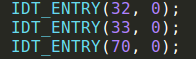
\includegraphics[width=\linewidth]{ejercicio5/idt.png}
\endminipage
\end{center}
\end{figure}

Ademas, las definimos en isr.h, para luego escribir su rutina.


\subsection{Ítem b): Rutina del reloj}

